\documentclass[11pt]{article}

%----- Do not change the values below -----%
\usepackage[numbers]{natbib}
\usepackage{geometry}
\geometry{tmargin=3cm, bmargin=2.2cm, lmargin=2.2cm, rmargin=2cm}

%----- Packages -----%
\usepackage{graphicx}   % For figures
\usepackage{lipsum}     % Dummy text (can be removed)
\usepackage{pdfpages}   % For inserting PDF appendices
\usepackage{amsmath}    % For math equations
\usepackage{hyperref}   % For clickable links in TOC and references

%----- Start Document -----%
\begin{document}

%----- Title Page -----%
\newgeometry{top=1.8cm, bottom=0.8cm, left=1.8cm, right=1.8cm}
\thispagestyle{empty}
\begin{figure}[h]
    
\includegraphics[width=11.20cm]{KUL_logo.jpg}
    \vfill
    
\includegraphics[width=11.20cm]{company_logo.png}
    \vfill
    \vspace*{5mm}
    Faculteit Ingenieurswetenschappen\\
    \textbf{Departement Werktuigkunde}\\
    Celestijnenlaan 300 - bus 2420 - B-3001 Heverlee\\
\end{figure}
\vspace*{2cm}

\begin{center}
    \Large{H01P7A: Ontwerpen in de werktuigkunde: industrieel project} \\ 
    \vspace*{3cm}
    \Huge\textbf{Project Titel}\\
    \vfill
\end{center}

\noindent % Suppress paragraph indentation
\begin{minipage}[t]{0.5\textwidth}
    \raggedright % Left align
    2024-2025 Bekaert Team *teamNr* 
\end{minipage}%
\begin{minipage}[t]{0.5\textwidth}
    \raggedleft % Right align
    Student1 (name + r-number) \\
    Student2 (name + r-number)\\
    Student3 (name + r-number) \\
    Student4 (name + r-number)\\
\end{minipage}
\vspace{3cm}
\restoregeometry



%----- Abstract -----%
\pagenumbering{roman}
\section*{Abstract}
\addcontentsline{toc}{section}{Abstract}

The abstract is not the same as the introduction. It should summarize your project clearly and concisely, including your objective, methods, and most important results (preferably with numbers). It must be self-contained and typically around 250 words.
\\ \\
\textbf{Poor example (vague):} \\
\textit{“We investigated possible grippers and evaluated them.”}
\\ \\
\textbf{Better example (specific):} \\
\textit{“A mechanical, pneumatic, and magnetic gripper were evaluated using a weighted decision matrix. The pneumatic gripper scored highest due to its low cost (€100) and sufficient load capacity of 1kg for this application.”}

%----- Table of Contents -----%
\newpage
\tableofcontents

%----- Main Content -----%
\newpage
\pagenumbering{arabic}
\setcounter{page}{1}

\section{Introduction}

Useful background on mechanical design principles can be found in \cite{PahlGerhard2007EDaSA, ChildsPeter2013MDEH}. For KU Leuven’s referencing guidelines, visit: \url{https://bib.kuleuven.be/training-en-tutorials/citeren}

This section should clearly define the problem or design challenge, the objectives of your project, and the context in which the work was carried out. Include only essential background, and focus on what the reader needs to know to understand the report.Conclude the introduction with a short summary of the report structure. 

The final report structure should look similar to:

\begin{itemize}
  \item \textbf{Chapters 1–4:} Revised content from the intermediate report (background, requirement analysis, and concept development).
  \item \textbf{Chapter 5:} Overview of the final selected concept.
  \item \textbf{Chapters 6–9:} Detailed analysis of key subsystems. Examples include:
  \begin{itemize}
    \item Structural analysis
    \item Mechanical calculations (e.g. load, stress, cycle time) $\rightarrow$ couple back to specifications/product!
    \item Kinematics/dynamics
    \item Material selection
    \item Power and energy consumption
    \item Motor/actuator selection
     \item ...
  \end{itemize}
  \item \textbf{Chapters 10–11:} Conclusions, evaluation, and recommendations, including:
  \begin{itemize}
    \item System advantages and disadvantages
    \item Cost analysis
    \item Safety and risk assessment
    \item ...
  \end{itemize}
\end{itemize}

\newpage
\section{Second Chapter Title}

You can begin each chapter with a short paragraph summarizing what it will cover. This helps the reader follow the report's structure.

\subsection{First Subsection Title}
\lipsum[3]

\subsubsection{Subsubsection Title}
Avoid making levels deeper than subsubsection (e.g., 2.1.1.1). If needed, restructure your content or use bullet points.

\subsection{Second Subsection Title}
\lipsum[13]

%----- References -----%
\clearpage
\renewcommand{\refname}{References}
\addcontentsline{toc}{section}{References}
\bibliographystyle{IEEEtran}
\bibliography{references}

%----- Appendices -----%
\clearpage
\appendix
\pagenumbering{roman}
\setcounter{page}{1}   % Optional: restart numbering from i

\section{Appendix Title}
Appendices can include technical drawings, data sheets, simulations, or detailed calculations. You can also insert complete documents using:
\begin{verbatim}
\includepdf[pages=-]{filename.pdf}
\end{verbatim}

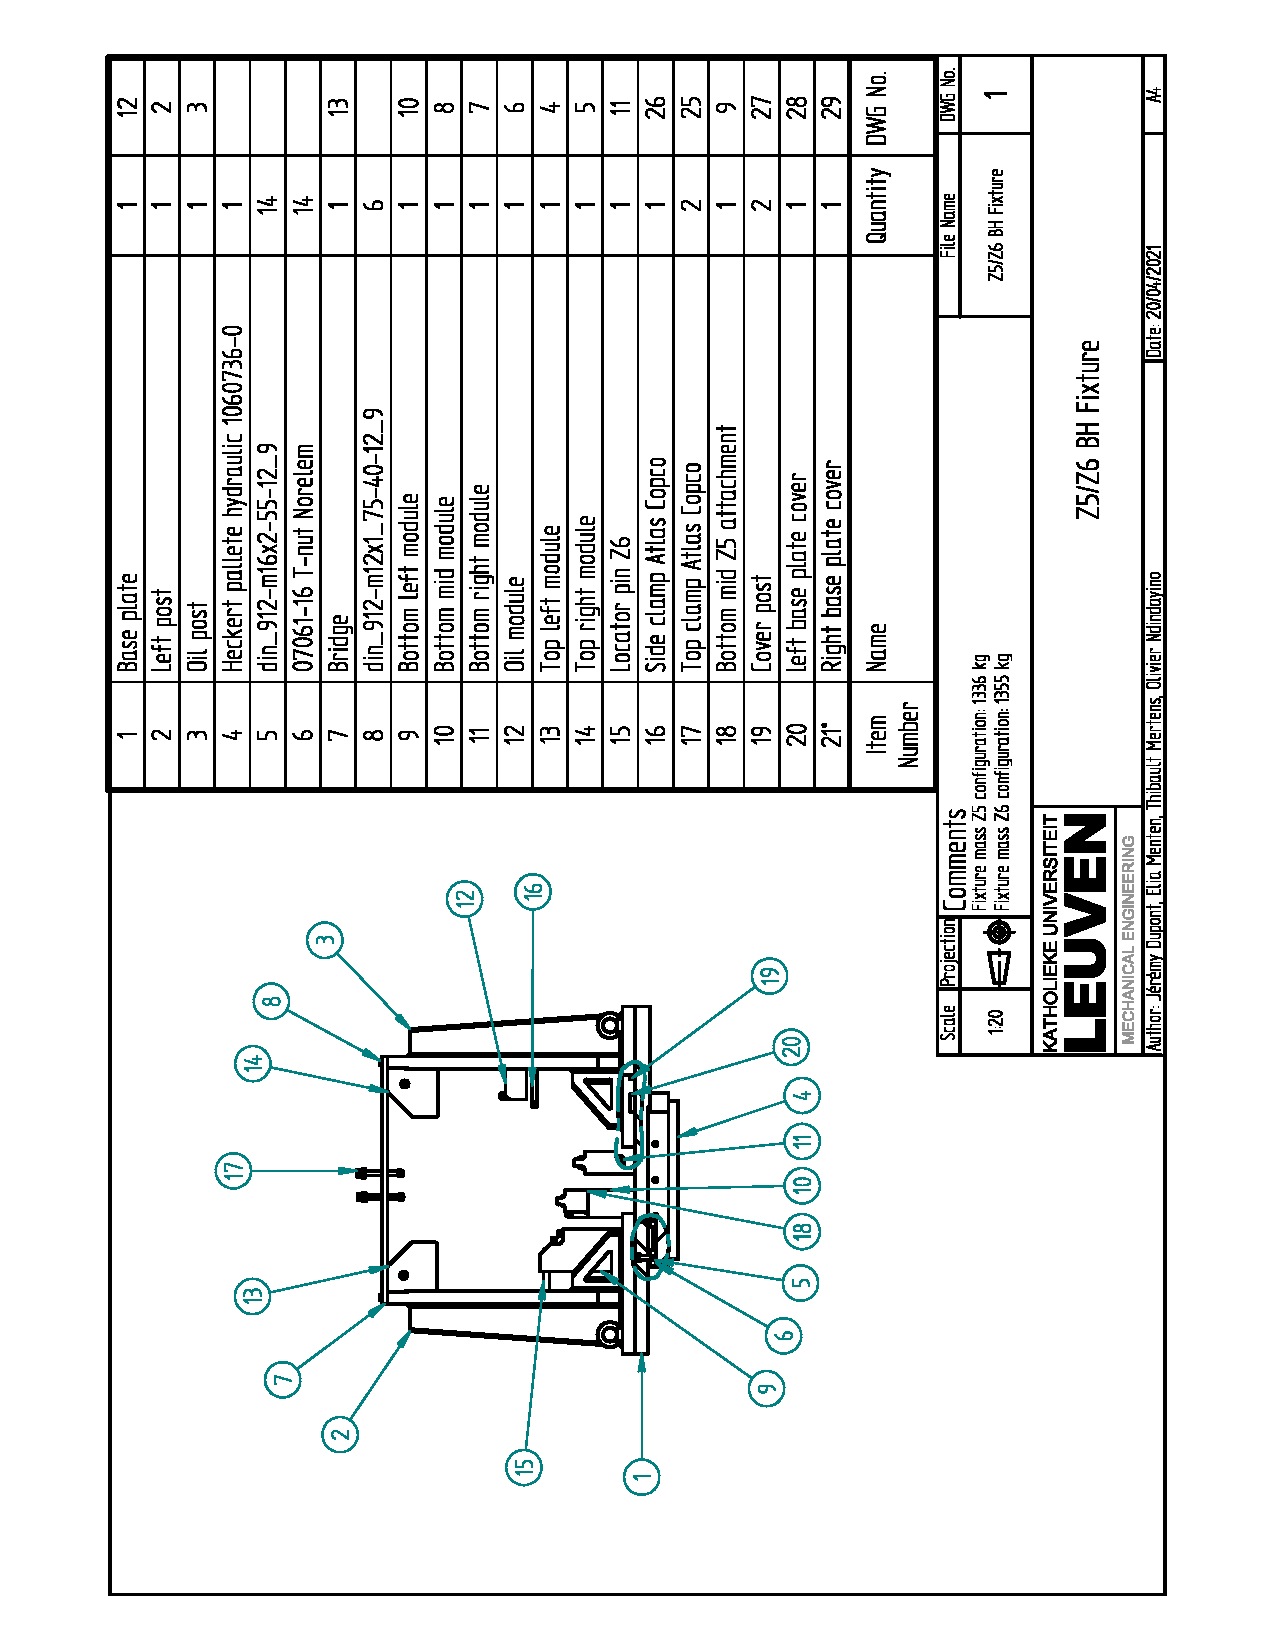
\includepdf[pages=-]{technical drawing example.pdf}

\end{document}
